\section{Key Features through A Running Example}
\label{sec:shors}

\begin{figure}[t]
{\small
\[\hspace*{-1em}
\begin{array}{r l  l}
\textcolor{blue}{1}
&&
\{A(x) * A(y) * B \}
\quad\text{where}\;\;
A(\beta) = \beta[0..n] \mapsto \ket{\overline{0}} 
\\[0.2em]
&&
\qquad\qquad\qquad
\qquad\qquad\quad
\begin{array}{l}
B = 1 < a < N \wedge n > 0 \;\wedge
\\\qquad N < 2^n \wedge \texttt{gcd}(a,N)=1
\end{array}
\\[0.5em]
\textcolor{blue}{2}
&
&
\textcolor{teal}{
\Rightarrow
\{\dabs{\ihadh}(x[0..n]) \mapsto C * A(y) * B \}
}
\\[0.2em]
&&
\qquad\qquad\qquad
\qquad\;\;
\text{where}
\;\;
\textcolor{teal}{
C = \shad{2^n}{n}{}
}
\\[0.5em]
\textcolor{blue}{3}
& \ssassign{x}{}{\ihadh};
&
\textcolor{teal}{
\{x[0..n] \mapsto C * A(y) * B \}
}
\\[0.4em]
\textcolor{blue}{4}
&
&
\textcolor{teal}{
\Rightarrow
\{x[0..n] \mapsto C * \dabs{y\splus 1}(y[0..n]) \mapsto \ket{\overline{0}.1} * B \}
}
\\[0.4em]
\textcolor{blue}{5}
& \ssassign{y}{}{y\splus 1};
&
\textcolor{teal}{
\{x[0..n] \mapsto C * y[0..n] \mapsto \ket{\overline{0}.1} * B \}
}
\\[0.4em]
\textcolor{blue}{6}
& 
&
\textcolor{teal}{
\Rightarrow
\{ E(0) * B \}
}
\;\;
\texttt{where}\;\;
\textcolor{teal}{E(k) =}
\\[0.2em]
&&
\qquad\qquad\quad\;
\qquad
\textcolor{teal}{
\begin{array}{l}
x[0..n\,\sminus\,k] \mapsto \shad{2^{n \,\sminus\,  k}}{n \,\sminus\, k}{}\;*
\\[0.2em]
\{x[0..k],y[0..n]\} \mapsto \sch{2^k}{\frac{1}{\sqrt{2^k}}}{\tos{j}.\tos{a^{j}\;\%\;N}}
\end{array}
}
\\[0.4em]
\textcolor{blue}{7}
&\sqforh{\sint{j}{0}}{j\,\slt\, n}{x[j]}{\dplus{j}}
&
\{E(j) * B \}
\\[0.4em]
\textcolor{blue}{8}
&
\{\quad  \ssassign{y}{}{a^{2^j}y\;\%\; N}
&
\textcolor{teal}{
\{E(j\,\splus\, 1) * B \}
}
\\[0.4em]
\textcolor{blue}{9}
&
\}
&
\textcolor{teal}{
\{E(n) * B \}
}
\\[0.4em]
\textcolor{blue}{10}
&
&
\textcolor{teal}{
\Rightarrow
\{\{x[0..n],y[0..n]\} \mapsto \sch{2^{n}}{\frac{1}{\sqrt{2^{n}}}}{\tos{j}.\tos{a^{j}\;\%\;N}} * B \}
}
\\[0.4em]
\textcolor{blue}{11}
& \sexp{u}{\smea{y}}{...}
&
\textcolor{purple}{
\big{\{}
\begin{array}{l}
x[0..n] \mapsto \smch{\frac{1}{\sqrt{s}}}{s}{t\,\splus\,k p} 
\wedge
p = \texttt{ord}(a,N)
\\
\wedge\;
\texttt{nat}(u)=a^{t}\;\%\;N
\wedge
s=\texttt{rnd}(\frac{2^n}{p}) \wedge B
\end{array}
\big{\}}
}
\end{array}
\]
}
\caption{First half of the Shor's algorithm quantum part. Second half in \Cref{fig:shorqafny2}. $\snat{u}$ gets the integer number part of $u$ (mode $\mmode$). $\sord{a,N}$ gets the order of $a$ and $N$. $\srnd{r}$ rounds $r$ to the nearest integer. }
\label{fig:shorqafny}
\end{figure}

As an illustration of QNP, we implement and prove part of the Shor's algorithm in \Cref{fig:shorqafny}.
Given an integer $N$, Shor's algorithm finds its nontrivial prime factors, which has the following step: (1) randomly pick a number $1 < a < N$ and compute $k=\texttt{gcd}(a,N)$ \footnote{compute the greatest common divisor of $a$ and $N$}; (2) if $k \neq 1$, $k$ is the factor; (3) otherwise, $a$ and $N$ are coprime and we find the order $p$ of $a$ and $N$ \footnote{the order $p$ is the smallest number such that $a^p \% N = 1$}; (4) if $p$ is even and $a^{\frac{p}{2}} \neq -1 \% N$, $\texttt{gcd}(a^{\frac{p}{2}}\pm 1,N)$ are the factors, otherwise, we repeat the process. Step (2) is the quantum part of Shor's algorithm and \Cref{fig:shorqafny} and \Cref{fig:shorqafny2} show its automated proof in QNP. In \Cref{fig:shorexample}, we show the actual implementation and proof in the Qafny tool.

\begin{wrapfigure}{r}{8.2cm}
  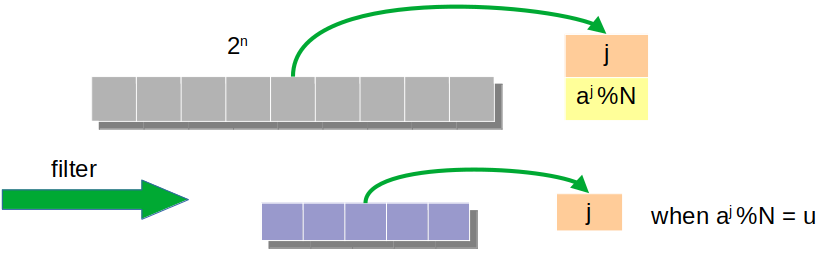
\includegraphics[width=.60\textwidth]{shorsmap}
  \caption{The array analogy of Shor's first half in \Cref{fig:shorqafny}. }
\label{fig:shorsanalog}
\end{wrapfigure}

The Shor's quantum first half in \Cref{fig:shorqafny} can be analogized as an efficient array filter operation.
The steps before line 11 (steps at line 3, 4 and 7-9) create a $2^n$-length of pairs, each of which is formed as $(j,a^j \% N)$ where $j\in [0,2^n)$. The measurement in line 11 filters the array as a new one ($x$) with all elements $j$ satisfying $a^j \% N=z$ where $z$ is a randomly picked number. Notice that modulo multiplication $f(j)=a^j\%N$ is a periodic function. All elements in $x$ satisfy $a^j \% N=z$, which means that 1) there will be a smallest $t$ such that $a^t \% N=z$, and 2) all elements can be rewritten as $j=t+kp$ and $p$ is the period of the modulo multiplication function because $a^{t+kp} \% N=z$, which is given as the post-condition on the right of line 11.
The first half implementation and correctness proof in \Cref{fig:shorqafny} exactly reflects the array analogy aspect.
One of the biggest advantage of using \qafny is that we can analogize quantum operations to classical array operations, so that we can utilize the existing automated proof infrastructure in many tools, such as Dafny.
In the Qafny implementation, verifying a quantum program usually requires only the user input of the pre-, post-, and loop invariant. For example, the proof of \Cref{fig:shorqafny} in \qafny requires none of the states marked teal, but only the conditions marked black and purple. \footnote{The purple is also not needed if we combine the Shor's first and second half algorithms together.}
Here, we step by step discuss the states, program syntax, and proofs of the aspect.

\begin{figure}[t]
{
  \small
\[\hspace*{-0.5em}
\begin{array}{l}
\textcolor{blue}{\text{Basic Terms:}}\\[0.2em]
\begin{array}{llcl llcl llcl}
\text{Nat. Num} & m, n & \in & \mathbb{N}
&
      \text{Real} & r & \in & \mathbb{R}
&
      \text{Complex Number} & z & \in & \mathbb{C}
\\
      \text{Variable} & x,y &&

 & \text{Bit} & d & ::= & 0\mid 1       
&
      \text{Bitstring} & c & \in & d^{+}      
\\
\text{Phase} & \alpha(r) & ::= & e^{2\pi i r}
\\
\end{array}
\\[1em]
\textcolor{blue}{\text{Modes, Kinds, Types, and Classical/Quantum Values:}}\\[0.2em]
\begin{array}{llclll} 
      \text{Mode} & g & ::= & \cmode  \mid \mmode\\
      \text{Classical Value} & v & ::= & n \mid (r,n)\\
      \text{Full Mode (Kind)} & \overline{g} & ::= & g \mid \qmode{n} \\
      \text{Quantum Type} & \tau & ::= & \tnort &\mid \thadt & \mid \tcht \\
      \text{Quantum Value} & q & ::= & \ket{c} & \mid \shad{2^n}{n}{\alpha(r_j)} &\mid \sch{m}{z_j}{c_j \,\beta_j} \\
    \end{array}
\\[1em]
\textcolor{blue}{\text{Quantum Sessions, Environment, and States}}\\[0.2em]
\begin{array}{llclcl} 
      \text{Range} & l & ::= & x[n..m] \\
      \text{Session} & \lambda & ::= & \overline{x[n..m]} & \text{by} & \uplus \\
      \text{Type Environment} & \sigma & ::= & \overline{\lambda : \tau } & \text{by} & \cup \\
      \text{Quantum State} & \varphi & ::= & \overline{ \lambda : q } & \text{by} & \cup \\
    \end{array}
\end{array}
  \]
}
  \caption{\qafny element syntax. Each range $x[n..m]$ in a session $\overline{x[n..m]}$ represents the number range $[n,m)$ in a qubit array $x$. Sessions are finite lists, while type environments and states are finite sets. the operations after "by" refer to the concatenation operations for session, type environments and quantum states. }
  \label{fig:qafny-state}
\end{figure}


